% Preamble
\documentclass[12pt]{article}
\usepackage{graphicx}
\usepackage{listings} % For code listing
\usepackage{hyperref}

% Packages
\usepackage{amsmath}
\usepackage{amssymb}
\usepackage{amsthm}
\usepackage{geometry}
\usepackage{setspace}
\usepackage{xcolor}
\usepackage{enumitem}

% Custom colors for code highlighting
\definecolor{codegreen}{rgb}{0,0.6,0}
\definecolor{codegray}{rgb}{0.5,0.5,0.5}
\definecolor{codepurple}{rgb}{0.58,0,0.82}
\definecolor{backcolour}{rgb}{0.95,0.95,0.92}

% Style for code
\lstset{
    language=C,
    backgroundcolor=\color{backcolour},
    commentstyle=\color{codegreen},
    keywordstyle=\color{magenta},
    numberstyle=\tiny\color{codegray},
    stringstyle=\color{codepurple},
    basicstyle=\ttfamily\small,
    breakatwhitespace=false,
    breaklines=true,
    captionpos=b,
    keepspaces=true,
    numbers=left,
    numbersep=5pt,
    showspaces=false,
    showstringspaces=false,
    showtabs=false,
    tabsize=2
}

% Set up the page margins
\geometry{left=0.5in,right=0.5in,top=0.5in,bottom=0.75in}

% Document
\begin{document}

\title{Analysis of Forking Processes in a UNIX Environment}
\author{Abraham J. Reines}
\date{\today}

\maketitle

\begin{abstract}
This report explains the process of executing a program intended to demonstrate the forking of processes in a UNIX environment. Running a C program to create multiple processes using the forking command and system calls facilitated an undertanding of differences between on-screen and redirect output to files with and without the use of \texttt{fflush(stdout)}. The findings are the technicalities of process managemetn in concurrent systems. This is a good example of the use of buffer management in output behavior. 
\end{abstract}

\section{Introduction}
The process of forking is fundamental in UNIX and POSIX-compliant operating systems. This report aims to explore the behavior of the fork system call and its implications on process management and output buffering.

\section{Definitions}

\begin{itemize}
    \item \textbf{fork:} The \texttt{fork} system call is used in Unix and Unix-like operating systems to create a new process. The newly created process is referred to as the child process, which is an exact duplicate of the calling process, known as the parent process, except for the returned value. It is a common way of splitting the control flow into two nearly identical processes which run concurrently in separate memory spaces.
    \item \textbf{getpid:} The \texttt{getpid} function returns the process identifier (PID) of the calling process. This is a unique number used by the system to identify a process. The PID can be used for various purposes, such as sending signals to the process to control its execution.
    \item \textbf{getppid:} The \texttt{getppid} function returns the parent process identifier (PPID), which is the PID of the process which created the calling process using \texttt{fork}. This can be used to establish a hierarchy of processes in a multi-process application.
\end{itemize}

\section{Methodology}
The C program is compiled and executed on a UNIX system. The output is observed on-screen, redirected to a file, and appended to analyze the behavior of process output under different conditions.

\section{Code Explanation}
The C program uses the \texttt{fork()} call. This is fundamental in craeting child processes in UNIX. \texttt{fork()} call results in the current process being duplicated. This creates a child process and a new process ID. The child process inherents a copy of the parent's memory. Their states may diverage as execution progresses. \texttt{getpid()} and \texttt{getppid()} functions find the process ID for parent and child processes, and place the IDs in the output so the process lineage can be tracked. \texttt{fflush(stdout)} makes sure the output buffer is flushed nice and fast, affecting the order and visibility of the output across different processes.
%\footnote{See next page for the full code listing.} 

\subsection{With fflush}
The use of fflush(stdout) ensures the output buffer is flushed after each print statement, which affects how often the output is written to the terminal or file. 

\lstinputlisting[language=C]{forking.c}

\subsection{Without fflush}
Commenting out the fflush(stdout) statement changes the program's behavior due to the output buffer not being manually flushed after each print statement.

\lstinputlisting[language=C]{forking_no_fflush.c}

\newpage
  \section{Results and Analysis}
This section will include the screenshots of the terminal output and the contents of the output files to illustrate the effects of forking and output buffering.

%\newpage
  \subsection{Terminal Output with fflush}
    \begin{figure}[h]
    \centering
    \includegraphics[width=\textwidth]{Screenshot 2024-02-16 at 10.49.48 AM.png}
    \caption{Terminal output when fflush is used.}
    \end{figure}

\subsection{Terminal Output without fflush}
\begin{figure}[h]
\centering
\includegraphics[width=\textwidth]{Screenshot 2024-02-16 at 10.50.28 AM.png}
\caption{Terminal output when fflush is not used.}
\end{figure}

\subsection{Text File Output with fflush}
\begin{figure}[h]
\centering
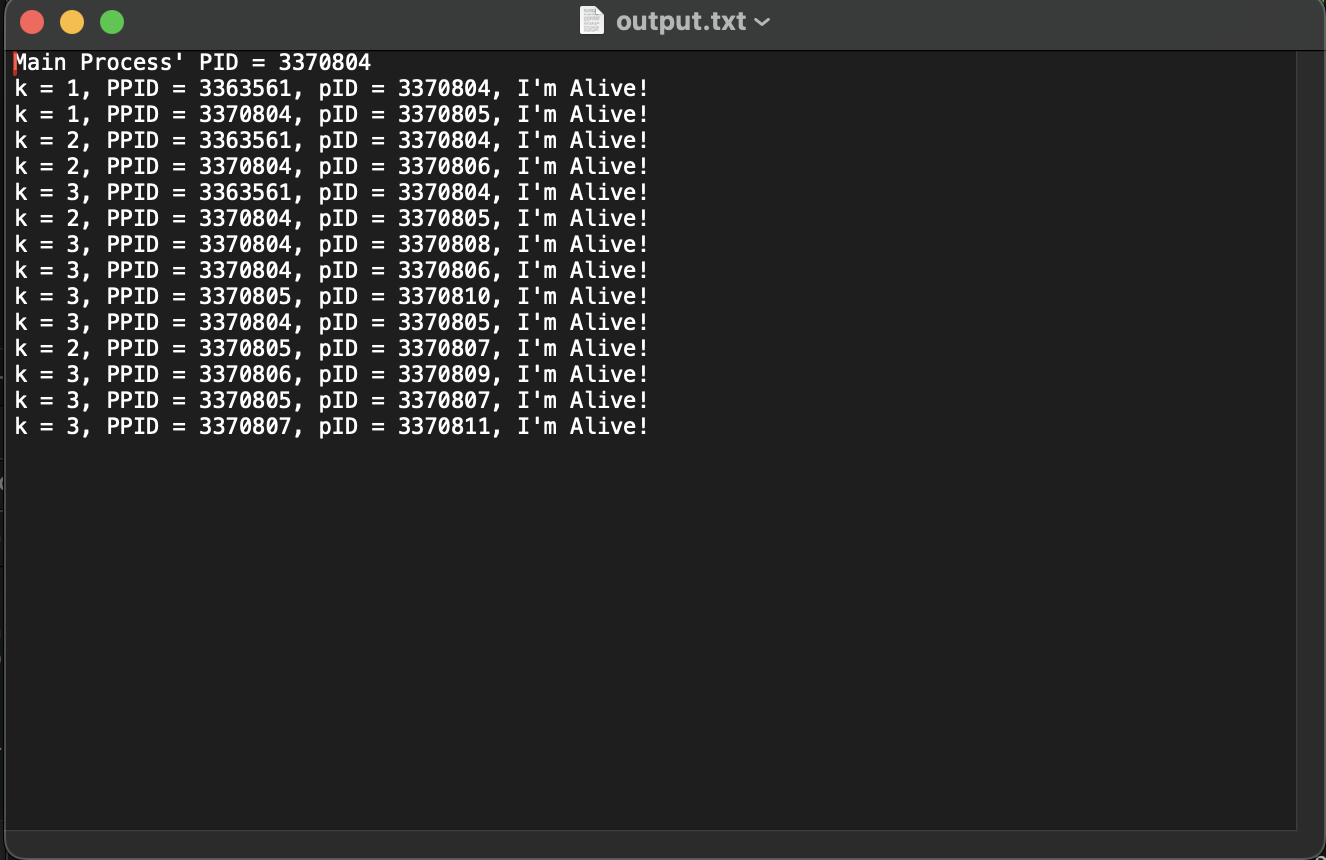
\includegraphics[width=\textwidth]{output_with_fflush.png}
\caption{File Output when fflush is used.}
\end{figure}

\newpage
  \subsection{Text File Output without fflush}
  \begin{figure}[h]
    \centering
    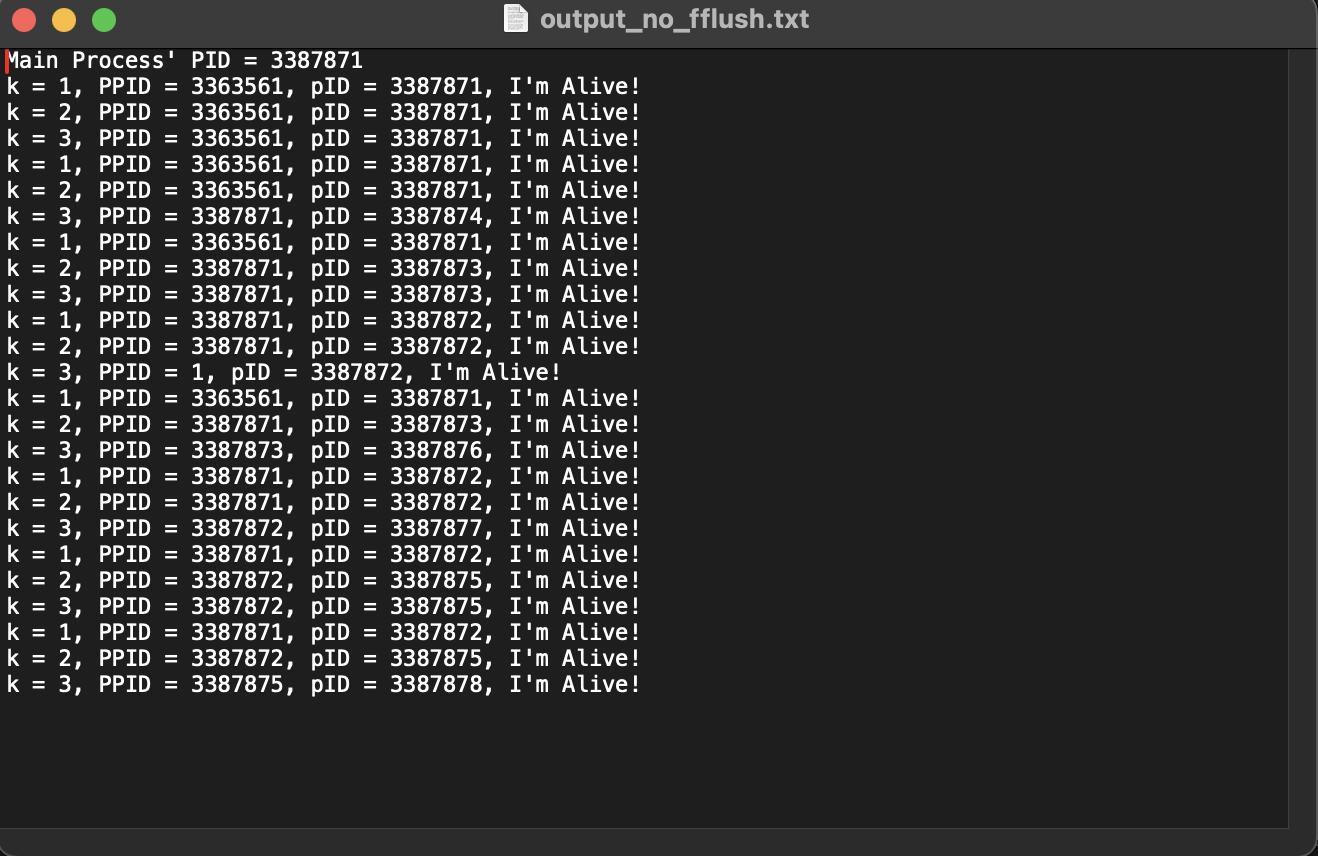
\includegraphics[width=17cm]{output_no_fflush.png}
    \caption{File Output when fflush is not used.}
  \end{figure}

\newpage
\subsection{File Output appended with fflush}
\begin{figure}[h]
\centering
\includegraphics[width=16cm]{Screenshot 2024-02-17 at 9.23.19 AM.png}
\caption{File output when fflush is used.}
\end{figure}

\newpage
\subsection{File Output appended without fflush}
\begin{figure}[h]
\centering
\includegraphics[width=14cm]{Screenshot 2024-02-17 at 9.23.39 AM.png}
\caption{File output when fflush is not used.}
\end{figure}

\newpage
  \subsection{Discussion}
The C program executed using the \texttt{fork()} system call on our machine. The behavior/output of the script is varied, based on \texttt{fflush(stdout)}, and the redirection methods we used. 

When \texttt{fflush(stdout)} was included, the output was consistently flushed to the terminal or file, ensuring the "I'm Alive!" message from both the parent and child processes was displayed immediately on our machine. The total count of displayed messages was \textit{14} when output to the terminal and directed to a file with "\texttt{> output.txt}". When appending to a file multiple times using "\texttt{>>}", the count did not vary; remaining \textit{14} lines.

Without \texttt{fflush(stdout)}, the behavior was different on our machine. The output was buffered, creating an inconsistent output message.This is due to the buffer not being flushed immediately, but rather automatically, when the program is terminated and/or the buffer is filled. The terminal output seemed to be \textit{14} lines, but the redirected/appended output was longer, about \textit{24} lines...

These variations show the effect of buffering in forking in our assignment. The parent and child processes have separate buffers when \texttt{fflush(stdout)} is ommitted. The \texttt{fflush(stdout)} line is important for predictable output in concurrent process execution. The disscrepancies between different execution environments (stu machine vs. other Linux mashines) further underscore the influence we experience when the operating system's process scheduling is working on our machine.

\subsection{With \texttt{fflush(stdout)}}
The program was run with the \texttt{fflush(stdout)} statement included, which forces the buffer to send the output to the terminal or file immediately. The counts for the display of "I'm Alive!" are as follows:
\begin{itemize}
  \item Displayed on-screen: 14 times.
  \item Redirected to a file using \texttt{>} operator: 14 times, as confirmed by \texttt{output.txt}.
  \item Appended to a file using \texttt{>>} operator, thrice: 42 times, aligning with expectations for two sequential appends.
\end{itemize}

\subsection{Without \texttt{fflush(stdout)}}
Omitting \texttt{fflush(stdout)}, hence relying on the system's buffering, led to the following outcomes:
\begin{itemize}
  \item Displayed on-screen: 14 times.
  \item Redirected to a file using \texttt{>} operator: 24 times, as recorded in \texttt{output\_no\_fflush.txt}.
  \item Appended to a file using \texttt{>>} operator, thrice: A varying larger number of messages were captured, suggesting the system's buffer was not flushed upon each program completion.
\end{itemize}

\subsection{Terminal Output with \texttt{fflush(stdout)}}
The terminal output displayed a total of 14 "I'm Alive!" messages, indicating the buffer was flushed correctly after each message.

\subsection{File Output with \texttt{fflush(stdout)}}
The file \texttt{output.txt} contained 14 messages, consistent with the terminal output and indicative of immediate flushing to the file.

\subsection{Terminal Output without \texttt{fflush(stdout)}}
A total of 14 messages were output to the terminal, suggesting some messages were not immediately flushed and were potentially lost due to the program's termination before the buffer was automatically flushed.

\subsection{File Output without \texttt{fflush(stdout)}}
The file \texttt{output\_no\_fflush.txt} recorded 24 messages, more than the terminal output, which could be attributed to the file buffer being filled and flushed automatically, as apposed to immdeiatly, before the program's completion, thereby capturing more messages.

\subsection{Appending the Output}
The consistent number of lines when appending with \texttt{fflush(stdout)} indicates the output buffer is flushed to the file immediately. Every "I'm Alive!" message is written to the file before the next iteration of the loop begins. 

An inconsistent number of lines, between terminal and appended file, when appending without \texttt{fflush(stdout)}, indicates the buffer is not being flushed immediately. 

\section{Conclusion}
This excersize shows the impace of the fork system call on process craetion and managment. It also highlights the orole of output buffering int the visibilty of print statemtents to the terminal and files. 

\vfill
  \section*{Academic Integrity Pledge}
    {\color{red}\textit{“This work complies with the JMU honor code. I did not give or receive unauthorized help on this assignment.”}}

\end{document}
